\documentclass[11pt,a4paper]{article}
\usepackage[margin=25mm]{geometry}
\usepackage{amsmath,amssymb,mathtools}
\usepackage{graphicx}
\graphicspath{{../resources/}}
\usepackage{url}
\usepackage[hidelinks]{hyperref}
\renewcommand{\texttt}[1]{\nolinkurl{#1}}
\makeatletter\g@addto@macro\UrlBreaks{\do\-\do\_\do\/\do\.}\makeatother % break long file paths (replaces xurl)
\usepackage{booktabs}
\usepackage{enumitem}
\setlist[itemize]{nosep,leftmargin=*}
\setlist[enumerate]{nosep,leftmargin=*}
\newcommand{\R}{\mathbb{R}}
\newcommand{\T}{\mathsf{T}}
\newcommand{\source}[1]{\par\smallskip\noindent\textit{Source: #1.}\par\smallskip}

\title{EE6204 Systems Analysis\\\large Linear and Nonlinear Programming Notes}
\author{Course-note revision}
\date{Updated: 4 September 2026}

\begin{document}
\maketitle

\noindent\textbf{Sources.} \texttt{resources/lecture-01-04-linear-and-nonlinear-programming.pdf} (Lectures 1--4),
\texttt{resources/introduction-to-linear-programming.pdf}, and the Week~3 exercise class (\texttt{resources/week-03-transcript.txt} + handwritten solutions \texttt{resources/EE6204\_Exercises-part1.pdf}). These notes explain and consolidate the methods; they do not reproduce every numerical tableau or worked calculation in the slides.

\tableofcontents
\newpage

\section{Optimization language and modelling}

An optimization model chooses decision variables $x$ to make an objective as good as possible while respecting constraints.  In minimization form, a general nonlinear program (NLP) is
\begin{equation}
 \min_{x\in\R^n} f(x)\quad\text{s.t.}\quad h_i(x)=0\ (i=1,\ldots,m),\qquad g_j(x)\geq 0\ (j=1,\ldots,p).
\end{equation}
The \emph{feasible set} is the set of $x$ satisfying every constraint. A feasible $x^\star$ is globally optimal if $f(x^\star)\leq f(x)$ for every feasible $x$; it is locally optimal if this only holds in a feasible neighbourhood of $x^\star$.

Before choosing an algorithm, formulate the physical question carefully.
\begin{enumerate}
 \item Define decision variables, including units and permitted values.
 \item Express the performance measure as an objective (and state max/min explicitly).
 \item Translate explicit resource, balance, quality, and capacity conditions into constraints.
 \item Add implicit conditions: non-negativity, integrality, bounds, and any conservation laws.
 \item Check dimensions and signs. For example, ``at least a demand'' is normally $\geq$; ``cannot exceed capacity'' is normally $\leq$.
\end{enumerate}

\paragraph{Useful classification.} Problems may be constrained or unconstrained, linear or nonlinear, continuous or integer-valued, deterministic or stochastic, and single- or multi-objective.  The distinction matters: linear structure gives especially strong geometry and algorithms.
\source{\texttt{resources/introduction-to-linear-programming.pdf}, slides 2--18;\\ \texttt{resources/lecture-01-04-linear-and-nonlinear-programming.pdf}, slides 1--9.}

\section{Linear programming (LP)}
\subsection{Definition, geometry, and graphical solution}
A linear program has a linear objective and linear constraints, e.g.
\begin{equation}
 \max_x\ c^\T x\quad\text{s.t.}\quad Ax\leq b,\qquad x\geq0.
\end{equation}
Its feasible region is an intersection of half-spaces, hence convex. A set $S$ is convex when $\alpha x+(1-\alpha)y\in S$ for all $x,y\in S$ and $0\leq\alpha\leq1$.  This is important: when a finite optimum exists, an LP has an optimum at an \emph{extreme point} (corner) of its feasible polyhedron.

For two variables, draw every constraint boundary, use a test point to retain the permitted side, intersect the half-spaces, and evaluate the objective at feasible corners.  Equivalent objective level lines $c^\T x=z$ can be translated in the improvement direction until the final contact with the feasible region. This reveals three diagnostic cases:
\begin{itemize}
 \item \textbf{Infeasible:} the half-spaces have no common point.
 \item \textbf{Unbounded:} an improving feasible ray lets $z$ increase (or decrease) without limit.
 \item \textbf{Multiple optima:} an objective level line is parallel to a binding feasible edge, so every point on an optimal edge has the same value.
\end{itemize}
\textbf{Unbounded region $\neq$ unbounded objective.} A ``$\geq$''-constrained minimisation has a feasible region that runs to infinity, but the objective is usually bounded below and the optimum is a corner. E.g.\ $\min 2x_1+3x_2$ s.t.\ $x_1+x_2\geq4$, $x_1+3x_2\geq6$, $x\geq0$: corners $(0,4),(3,1),(6,0)$ give $12,9,12$, so $(3,1)$, $z=9$. Declare ``unbounded'' only if an improving move stays feasible all the way to infinity.

\paragraph{Example: product mix.} If $x$ suits and $y$ gowns use cotton, silk, and wool, a model is
\[
 \max\ 30x+50y\quad\text{s.t.}\quad 2x+y\leq16,\quad x+2y\leq11,\quad x+3y\leq15,\quad x,y\geq0.
\]
The model separates a value ($30x+50y$) from physical limits. If garments must be whole, add $x,y\in\mathbb{Z}_{\geq0}$: that is an integer LP, not an ordinary continuous LP.
\source{\texttt{resources/introduction-to-linear-programming.pdf}, slides 15--28; \texttt{resources/lecture-01-04-linear-and-nonlinear-programming.pdf}, slides 3--15 and 37--40.}

\subsection{Standard form and an initial basic feasible solution}
For the simplex method, write constraints as equalities with non-negative variables and right-hand sides. A convenient matrix form is
\begin{equation}
 \text{optimize }z=c^\T x\quad\text{s.t.}\quad Ax=b,\qquad x\geq0.
\end{equation}
Use the following transformations (after multiplying a constraint by $-1$ if needed to make its RHS non-negative):
\begin{align*}
 a_i^\T x &\leq b_i &&\Longrightarrow& a_i^\T x+s_i&=b_i,&s_i&\geq0 &&\text{(slack)},\\
 a_i^\T x &\geq b_i &&\Longrightarrow& a_i^\T x-e_i&=b_i,&e_i&\geq0 &&\text{(surplus)},\\
 x_k\text{ free}&&&\Longrightarrow&x_k&=x_k^+-x_k^-,&x_k^+,x_k^-&\geq0.
\end{align*}
An artificial variable $a_i\geq0$ is temporarily added to an equality or a surplus row that has no obvious basic variable. It creates an initial basic feasible solution (BFS), but is not part of the original model. The Big-$M$ device penalizes it by $+Ma_i$ in a minimization (or $-Ma_i$ in a maximization), where $M$ is very large; a valid solution to the original problem must drive every artificial variable to zero.

Let $A$ be $m\times n$ with rank $m$. Select $m$ linearly independent columns to form a basis $B$. Set the other $n-m$ \emph{nonbasic} variables to zero and solve $x_B=B^{-1}b$. This is a basic solution; it is a BFS only if $x_B\geq0$. BFSs are precisely the extreme points. A BFS is \emph{degenerate} if at least one basic variable is zero, which can cause a pivot with no movement in the original variables.
\source{\texttt{resources/lecture-01-04-linear-and-nonlinear-programming.pdf}, slides 16--40.}

\subsection{The simplex method}
Simplex moves from one BFS to an adjacent BFS while preserving feasibility and improving the objective. In a conventional tableau with a minimization reduced-cost row, the source's procedure is:
\begin{enumerate}
 \item Choose the most negative reduced cost as the entering (work-column) variable. If no reduced cost is negative, the current BFS is optimal for that tableau convention.
 \item Apply the minimum-ratio test $b_i/a_{ij}$ over rows with $a_{ij}>0$; its row gives the leaving variable. If no eligible row exists, the problem is unbounded in the improving direction.
 \item Pivot: scale the pivot row to make its pivot one, then use row operations to make the other entries in its column zero.
 \item Exchange the entering and leaving variables in the basis, and repeat.
\end{enumerate}
The sign convention in a tableau must be kept consistent; never mix a minimization reduced-cost test with a maximization one. The ratio test is what prevents a step from leaving the feasible region. A tie in the ratio test means the next BFS is degenerate (some basic variable becomes zero); either tied row is a valid pivot.

\paragraph{Special cases read off a tableau.} First fix basic (unit column, value $=$ its row's RHS) vs.\ nonbasic (value $0$). Then:
\begin{itemize}
 \item \textbf{Degenerate:} a \emph{basic} variable $=0$ (zero in a basic row's RHS).
 \item \textbf{Alternative optima:} tableau optimal \emph{and} a \emph{nonbasic} variable has reduced cost $0$ --- pivot it in to get another optimal vertex / a whole optimal edge. (A zero under a basic column is meaningless.)
 \item \textbf{Unbounded:} a nonbasic variable has negative reduced cost but no positive entry in its column (no ratio-test row).
\end{itemize}
Do not swap the first two: degeneracy is a \emph{basic variable value} at $0$; alternative optima is a \emph{nonbasic reduced cost} at $0$.

\paragraph{Two-phase method.} When artificial variables are needed, Phase I minimizes their total (or equivalently performs the source's auxiliary-row procedure) to seek a BFS with all artificials zero. A positive minimum means the original LP is infeasible. Remove artificial columns and the Phase-I row once they have left the basis, then optimize the original objective in Phase II. This avoids treating $M$ as a numerical finite constant.
\source{\texttt{resources/lecture-01-04-linear-and-nonlinear-programming.pdf}, slides 41--59.}

\section{Duality and sensitivity}
\subsection{Primal--dual pair and complementary slackness}
For the source's nonstandard primal minimization form,
\begin{equation}
 \min\ c^\T x\quad\text{s.t.}\quad Ax\geq b,\quad x\geq0,
\end{equation}
the symmetric dual is
\begin{equation}
 \max\ b^\T w\quad\text{s.t.}\quad A^\T w\leq c,\quad w\geq0.
\end{equation}
The coefficient matrix transposes; primal constraints become dual variables, and primal variables become dual constraints.  A minimization primal has a maximization dual in this pair. Strong duality says that if either problem has an optimum, the other does too and their optimal objective values agree.

At optimal primal $x^\star$ and dual $w^\star$, complementary slackness gives a compact diagnostic:
\begin{align*}
 w_i^\star\big((Ax^\star)_i-b_i\big)&=0 &&\text{for every primal constraint},\\
 x_j^\star\big(c_j-(A^\T w^\star)_j\big)&=0 &&\text{for every primal variable}.
\end{align*}
Thus, a strictly slack primal constraint has zero shadow price; a positive primal activity makes its dual constraint tight. In the LP setting, dual multipliers quantify the marginal value of relaxing/tightening resource right-hand sides, subject to the stated allowable range.

\paragraph{Dual as a dimensionality tool.} The dual has one variable per primal constraint. A problem with more than two variables but only two constraints has a two-variable dual that can be solved graphically; recover the primal optimum by complementary slackness. Count variables against constraints and graph whichever form has two variables.
\source{\texttt{resources/lecture-01-04-linear-and-nonlinear-programming.pdf}, slides 60--69; \texttt{resources/week-03-transcript.txt} (lecturer-stated quiz technique).}

\subsection{LP sensitivity analysis}
Sensitivity analysis asks whether a known optimum remains feasible and optimal after changing data $A$, $b$, or $c$, rather than resolving blindly.

With an unchanged basis $B$, a right-hand-side perturbation $b\mapsto b+\Delta b$ gives
\[
 x_B^{\mathrm{new}}=B^{-1}(b+\Delta b).
\]
The current basis remains primal feasible exactly when this vector is non-negative. For an objective-coefficient change, keep all reduced costs at their optimal sign. For a change to a column of $A$, recompute the affected tableau column and its reduced cost, then test both feasibility and reduced-cost optimality. The dual view gives the same idea: the current primal solution remains optimal if its associated dual vector is still feasible after the change.

\paragraph{Caution.} An allowable range says the \emph{basis} remains optimal; within it, objective values and basic-variable values can still change. Once a feasibility or reduced-cost test fails, pivot/re-optimise rather than extrapolating the old solution.
\source{\texttt{resources/lecture-01-04-linear-and-nonlinear-programming.pdf}, slides 70--90.}

\section{Special LP structures}
\subsection{Transportation problem}
Ship $x_{ij}\geq0$ units from source $i$ (supply $s_i$) to destination $j$ (demand $d_j$), at cost $c_{ij}$ per unit:
\begin{align*}
 \min\quad&\sum_i\sum_j c_{ij}x_{ij},\\
 \text{s.t.}\quad&\sum_jx_{ij}=s_i&&\forall i,\\
 &\sum_ix_{ij}=d_j&&\forall j,\\
 &x_{ij}\geq0.
\end{align*}
For a balanced model, $\sum_i s_i=\sum_jd_j$; otherwise add a dummy source/destination with the appropriate supply/demand (and stated dummy costs). A nondegenerate transportation BFS has $m+n-1$ basic allocations.

The transportation tableau exploits this structure. Obtain an initial BFS (the slides use Vogel's approximation method), calculate potentials $u_i,v_j$ for basic cells from $u_i+v_j=c_{ij}$, then test nonbasic cells using reduced costs $c_{ij}-u_i-v_j$. For minimization, all nonnegative values certify optimality. Otherwise select a negative cell, form an alternating $+/-$ closed loop through basic cells, and move the largest amount allowed by the cells marked $-$; this replaces one basic cell while preserving every row and column balance. A zero basic allocation is a degenerate case and needs careful bookkeeping to retain $m+n-1$ basis cells.
\source{\texttt{resources/lecture-01-04-linear-and-nonlinear-programming.pdf}, slides 65--80.}

\subsection{Assignment problem and Hungarian method}
Assign each of $n$ agents to exactly one of $n$ jobs. With $x_{ij}\in\{0,1\}$,
\[
 \min\sum_{i=1}^n\sum_{j=1}^n c_{ij}x_{ij},\qquad
 \sum_jx_{ij}=1,\quad\sum_ix_{ij}=1.
\]
If counts differ, add dummy agents/jobs, typically with zero cost when ``unassigned'' is a valid interpretation. Prohibited assignments can be represented by a sufficiently large penalty cost, with its modelling meaning stated explicitly.

The Hungarian method for a minimization cost matrix is:
\begin{enumerate}
 \item Subtract each row minimum and then each column minimum.
 \item Cover all zeros with the fewest horizontal/vertical lines. If $n$ lines suffice, choose $n$ independent zeros (no shared row/column) for the assignment.
 \item Otherwise, subtract the smallest uncovered value from every uncovered entry and add it to every doubly covered entry; leave singly covered entries unchanged. Repeat the covering test.
\end{enumerate}
Row/column reductions preserve relative assignment costs because every complete assignment uses exactly one item from each row and column.
\source{\texttt{resources/lecture-01-04-linear-and-nonlinear-programming.pdf}, slides 81--90. In the Week~3 transcript the lecturer states the Hungarian/assignment method is tested in \emph{neither} Quiz~1 nor the final exam.}

\subsection{Integer linear programming}
If variables must be integers, dropping that requirement gives the \emph{LP relaxation}, whose optimal value bounds the integer optimum (from above, for a maximization). Rounding the relaxed solution is not valid --- it may be infeasible or suboptimal.
\begin{itemize}
 \item \textbf{Two variables:} solve graphically, then slide the objective line to its last contact with an integer lattice point inside the relaxed region. Show the value line and contact point; do not enumerate lattice points for marks.
 \item \textbf{Branch and bound:} solve the relaxation; if $x_k=f$ is fractional, branch into $x_k\leq\lfloor f\rfloor$ and $x_k\geq\lceil f\rceil$ and recurse. Prune a node that is infeasible, bounded no better than the incumbent integer solution, or itself integer (then update the incumbent).
\end{itemize}
Example: $\max 7x_1+5x_2$ s.t. $4x_1+6x_2\leq18$, $2x_1+6x_2\leq9$, $6x_1+3x_2\leq27$, $x\geq0$ integer. Relaxation $(4.5,0)$, value $31.5$; branching $x_1\leq4$ then $x_2\leq0$ gives the integer optimum $(4,0)$, value $28$ (the $x_1\geq5$ branch is infeasible, the $x_2\geq1$ branch is bounded at $15.5$).
\source{\texttt{resources/EE6204\_Exercises-part1.pdf}, Q3 (tree completed for these notes); \texttt{resources/week-03-transcript.txt}. Not in the lecture deck. Quiz~1: expect the graphical lattice method only; branch and bound is final-exam material.}

\section{Nonlinear programming (NLP)}
\subsection{One-dimensional search and Newton's method}
For an unconstrained scalar minimization $\min_{x\in[a,b]}f(x)$, region-elimination methods assume the relevant interval is \emph{unimodal}: it has one local/global valley (reverse comparisons for maximization). Given $x_1<x_2$, if $f(x_1)<f(x_2)$, discard the right portion beyond $x_2$; if $f(x_1)>f(x_2)$, discard the left portion before $x_1$.

Fibonacci search chooses interior points using Fibonacci ratios when the permitted final interval length is specified. Golden-section search uses the fixed ratio $\tau=(\sqrt5-1)/2\approx0.618$ so that one old evaluation becomes a new interior point after every reduction. Stop once the bracket is within the prescribed tolerance; report an estimated optimizer and the final uncertainty interval, not false precision.

Newton's scalar stationary-point iteration is
\[
 x_{k+1}=x_k-\frac{f'(x_k)}{f''(x_k)}.
\]
It is fast near a regular optimum, but it requires $f''(x_k)\ne0$ and can fail or move to the wrong stationary point from a poor initial point. Verify the resulting point using $f''(x^\star)>0$ for a local minimum (or $<0$ for a local maximum).
\source{\texttt{resources/lecture-01-04-linear-and-nonlinear-programming.pdf}, slides 97--109.}

\subsection{Multivariable optimality and Newton step}
For differentiable $f:\R^n\to\R$, define
\[
 \nabla f(x)=\begin{bmatrix}\partial f/\partial x_1&\cdots&\partial f/\partial x_n\end{bmatrix}^{\T},\qquad
 H(x)=\nabla^2f(x).
\]
A necessary condition for an unconstrained interior local optimum is $\nabla f(x^\star)=0$. At a stationary point, $H\succ0$ implies a strict local minimum and $H\prec0$ a strict local maximum; an indefinite Hessian indicates a saddle. For symmetric $H$, positive definiteness can be checked from positive leading principal minors (Sylvester's criterion); negative definiteness requires alternating signs of those minors, beginning negative.

The multivariable Newton step solves the local quadratic model:
\[
 x_{k+1}=x_k-H(x_k)^{-1}\nabla f(x_k).
\]
In practice, an indefinite or badly conditioned Hessian may yield a non-descent step, so damping/line search or a modified Hessian is often needed. The slides distinguish derivative-free direct searches from gradient-based methods; the latter use gradient/Hessian information to construct a direction.
\source{\texttt{resources/lecture-01-04-linear-and-nonlinear-programming.pdf}, slides 110--119.}

\subsection{Equality constraints and Lagrange multipliers}
For $\min f(x)$ subject to $h_i(x)=0$, define
\[
 \mathcal{L}(x,\lambda)=f(x)+\sum_{i=1}^m\lambda_i h_i(x).
\]
At a regular local optimum (the equality-constraint gradients are linearly independent), solve
\begin{equation}
 \nabla_x\mathcal{L}(x^\star,\lambda^\star)=0,\qquad h(x^\star)=0.
\end{equation}
Stationarity says the objective gradient is balanced by constraint normals, so no feasible first-order direction improves the objective. It is necessary, not automatically sufficient.

For a second-order check, let $M=\{y:\nabla h_i(x^\star)^\T y=0,\ i=1,\ldots,m\}$ be the tangent subspace. If
\[
 y^\T\nabla^2_{xx}\mathcal{L}(x^\star,\lambda^\star)y>0\quad\text{for every nonzero }y\in M,
\]
then the regular point is a strict constrained local minimum. The restriction to $M$ is essential: curvature in directions that violate a constraint is irrelevant.
\source{\texttt{resources/lecture-01-04-linear-and-nonlinear-programming.pdf}, slides 120--128.}

\subsection{Inequality constraints, KKT, and convexity}
For the convention $g_j(x)\geq0$ in a minimization problem, use
\[
 \mathcal{L}(x,\lambda,\mu)=f(x)+\sum_i\lambda_i h_i(x)+\sum_j\mu_jg_j(x).
\]
Under a suitable constraint qualification (the slides assume a regular point), the Karush--Kuhn--Tucker (KKT) necessary conditions are
\begin{align*}
 \nabla_x\mathcal{L}(x^\star,\lambda^\star,\mu^\star)&=0 &&\text{(stationarity)},\\
 h_i(x^\star)&=0,\quad g_j(x^\star)\geq0 &&\text{(primal feasibility)},\\
 \mu_j^\star&\geq0 &&\text{(dual feasibility)},\\
 \mu_j^\star g_j(x^\star)&=0 &&\text{(complementary slackness)}.
\end{align*}
Complementary slackness means either an inequality is inactive ($g_j>0$) and its multiplier is zero, or the constraint is active ($g_j=0$) and may carry a nonzero marginal value. In hand solutions, enumerate plausible active sets, solve stationarity with the corresponding equalities, then reject candidates that violate any KKT condition.

Convexity turns these local conditions into a global certificate. For a minimization problem, if $f$ is convex, each equality is affine, each feasible-set inequality is concave in the $g_j\geq0$ convention, and an appropriate regularity condition holds, a feasible KKT point is globally optimal. Strict convexity of $f$ over the feasible set yields a unique optimizer. Do not claim global optimality from KKT alone in a nonconvex problem.
\source{\texttt{resources/lecture-01-04-linear-and-nonlinear-programming.pdf}, slides 129--140.}

\subsection{NLP sensitivity interpretation}
For a small RHS perturbation of an active constraint, the associated optimal Lagrange multiplier predicts the first-order change in optimal objective value, subject to the sign convention and a stable active set. This is the NLP analogue of an LP shadow price. The approximation is local: if the active set changes or regularity fails, re-solve the optimization problem.
\source{\texttt{resources/lecture-01-04-linear-and-nonlinear-programming.pdf}, slide 141.}

\section{Revision checklist}
\begin{itemize}
 \item Can I formulate variables, objective, constraints, domains, and units without reversing $\leq$/$\geq$?
 \item Can I turn every LP constraint into equality form and identify slack, surplus, artificial, basic, and nonbasic variables?
 \item Can I execute one simplex pivot, state the ratio-test restriction, and diagnose unboundedness/infeasibility?
 \item Can I build the symmetric dual and use complementary slackness to infer zeros/tight constraints, including dualising a $>2$-variable / 2-constraint LP to solve it graphically?
 \item Can I solve a two-variable integer LP on the graph and take one branch-and-bound step?
 \item Can I test whether an old LP basis remains feasible/optimal after changing $b$, $c$, or $A$?
 \item Can I run the transportation optimality test and explain the loop update, and apply the Hungarian reductions?
 \item Can I distinguish a stationary point from a certified local/global optimum and write the KKT system with a consistent inequality sign convention?
\end{itemize}

\appendix
\section{Week~3 exercise class --- source scans}
\label{app:exercises}
Handwritten worked solutions from the Week~3 exercise lecture (\texttt{resources/EE6204\_Exercises-part1.pdf}), for reference. The LPs are typeset and re-derived in \S2.3 and \S4.3. Q1's gradient annotation reads $[7;5]$ but should be $[5;7]$; the Q3 tree and the Q4--Q5 answers are completed in \S4.3 because the scan stops short.

\begin{figure}[p]\centering
 \fbox{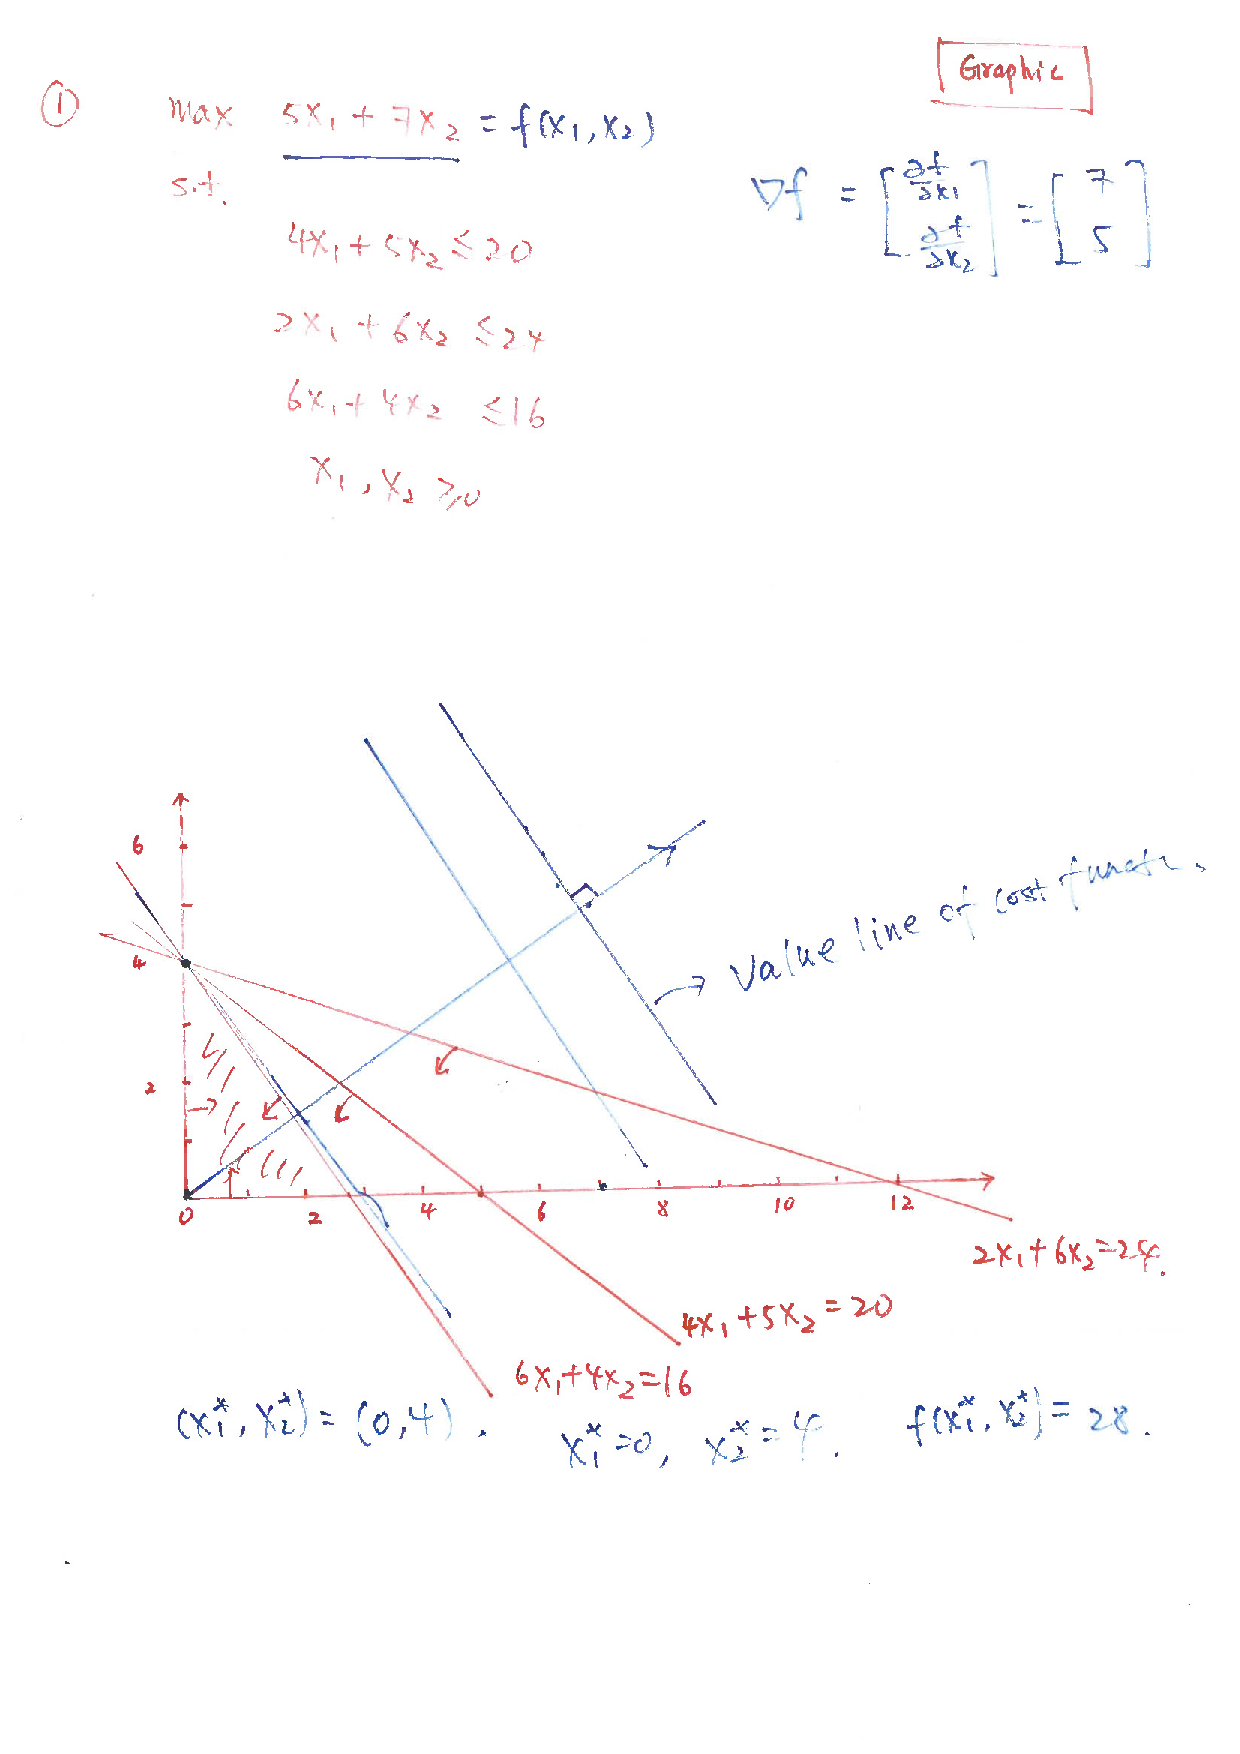
\includegraphics[page=1,width=0.72\linewidth]{EE6204_Exercises-part1.pdf}}
 \caption{Q1 graphical: $\max\ 5x_1+7x_2$ s.t.\ $4x_1+5x_2\leq20$, $2x_1+6x_2\leq24$, $6x_1+4x_2\leq16$ $\Rightarrow$ $(0,4)$, $f=28$ (degenerate --- all three lines through the optimum).}
\end{figure}
\begin{figure}[p]\centering
 \fbox{\includegraphics[page=2,width=0.72\linewidth]{EE6204_Exercises-part1.pdf}}
 \caption{Q2 simplex on the same LP: three-way ratio-test tie, degenerate optimal tableau, $z=28$.}
\end{figure}
\begin{figure}[p]\centering
 \fbox{\includegraphics[page=3,width=0.72\linewidth]{EE6204_Exercises-part1.pdf}}
 \caption{Q3 branch and bound: $\max\ 7x_1+5x_2$ s.t.\ $4x_1+6x_2\leq18$, $2x_1+6x_2\leq9$, $6x_1+3x_2\leq27$, integer $\Rightarrow$ $(4,0)$, $z=28$.}
\end{figure}
\begin{figure}[p]\centering
 \fbox{\includegraphics[page=4,width=0.72\linewidth]{EE6204_Exercises-part1.pdf}}
 \caption{Q4 graphical: $\max\ 200x+550y$ s.t.\ $100x+250y\leq5000$, $x+y\leq50$ $\Rightarrow$ $(0,20)$, value $11000$.}
\end{figure}
\begin{figure}[p]\centering
 \fbox{\includegraphics[page=5,width=0.72\linewidth]{EE6204_Exercises-part1.pdf}}
 \caption{Q5: the same LP as Q4, by the simplex method.}
\end{figure}

\end{document}
